\documentclass[12pt, a4paper]{article}
\usepackage[utf8]{inputenc}
\usepackage[portuguese]{babel}
\usepackage{geometry} % Pacote para gerenciar as margens e orientação
\usepackage{booktabs}
\usepackage{xcolor}
\usepackage{listings}
\usepackage{graphicx}
\usepackage{enumitem}
\usepackage{float} %

\geometry{landscape, margin=2.5cm}

\title{Requisitos de verificação}
\author{Matheus Grossi}
\date{2025}

\begin{document}
	
	\maketitle
	
	\vspace{3cm}
	\section{Identificação do Bloco}
	\begin{itemize}[label=\textbullet]
		\item \textbf{1.1. Nome do bloco:} Gerador de números pseudo-aleatórios de 3 bits com não repetição (RNG)
		\item \textbf{1.2. Versão:} 1.0
		\item \textbf{1.3. Autor do bloco:} Matheus Grossi
		\item \textbf{1.4. Responsável pela verificação:} Matheus Grossi.
		\item \textbf{1.5. Ferramentas utilizadas:} UVM + Verilator + GTKWave
		\item \textbf{1.6. Data do início e término:} 24/02/2026 - 10/03/2026
	\end{itemize}
	
	
	\section{Arquivos da bancada}
	\begin{figure}[H]
		\centering
		\fbox{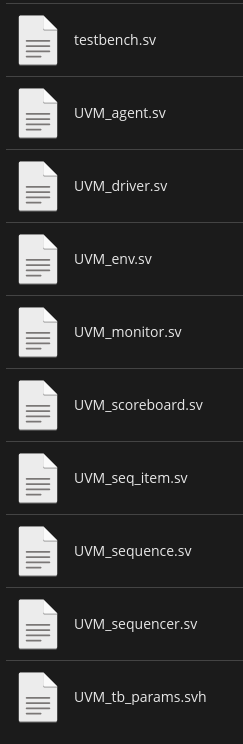
\includegraphics[width=0.17\textwidth]{UVM.png}}
		\caption{Lista de itens que compõem a bancada}
	\end{figure}
	
	
	\section{Objetivo da Verificação}
	O objetivo da verificação do bloco é assegurar que:
	\begin{itemize}
		\item O protocolo de solicitação e aceite do bloco (\texttt{req\_num\_i} e \texttt{wr\_i}) ocorra conforme o handshake modelado na bancada;
		\item O monitor capture corretamente as amostras válidas de \texttt{num\_to\_send\_o} na presença de \texttt{wr\_i};
		\item O scoreboard consolide a sequência observada, contabilize ocorrências e sinalize repetições reais;
		\item \textbf{Robustez temporal:} o bloco seja exercitado sob três faixas de temporização configuradas na sequência (\texttt{clk\_toggle\_tu} = 3, 7 e 10), com espaçamentos pseudoaleatórios entre requisições.
	\end{itemize}
	
	\section{Casos de Teste Executados}
	% DICA: Como a página agora é larga, usei \centering para centralizar a tabela.
	% Se quiser que a tabela ocupe a largura total, considere usar o pacote 'tabularx'.
	\begin{table}[h!]
		\centering
		\small
		\begin{tabular}{|p{4cm}|p{5cm}|p{4cm}|p{4cm}|p{4cm}|}
			\hline
			\textbf{ID do Teste} & \textbf{Descrição} & \textbf{Sequência Principal} & \textbf{Ambiente} & \textbf{Critério de Sucesso} \\ \hline
			rng\_test & Teste principal com 24 rodadas, divididas em três faixas temporais, com intervalos pseudoaleatórios entre requisições. O teste valida o handshake, a captura das amostras pelo monitor e a consolidação da sequência observada no scoreboard. & \texttt{rng\_sequence} & \texttt{tb\_rng + rng\_env + rng\_agent + rng\_driver + rng\_monitor + rng\_scoreboard} & Execução completa das 24 rodadas, ausência de \texttt{uvm\_fatal}, publicação de amostras válidas pelo monitor e geração do resumo final do scoreboard com contagem consistente. \\ \hline
		\end{tabular}
	\end{table}
	
	\section{Resultados}
	\subsection{Sumário dos testes executados}
	\begin{itemize}
		\item \textbf{Total de sequências:} 1 sequência principal (\texttt{rng\_sequence})
		\item \textbf{Passaram:} 1 teste estrutural previsto pela bancada
		\item \textbf{Falharam:} 0 falhas estruturais explícitas na bancada
	\end{itemize}
	
	\subsection{Comportamentos esperados observados?}
	Sim, do ponto de vista estrutural da bancada. A verificação implementada observa corretamente a liberação de reset, a execução de 24 rodadas, a variação temporal do clock por item de sequência, a publicação de amostras pelo monitor quando \texttt{wr\_i} está ativo e a consolidação das ocorrências no scoreboard.
	
	\subsection{Comportamentos inesperados detectados?}
	Sim. Pela análise da bancada, foram identificadas limitações importantes:
	\begin{itemize}
		\item Uma falha no protocolo de hand-shaking foi detectado durante a verificação, mas após a execução de lint foi possível localizar os erros no RTL o que permitiu que pudêssemos resolver o problema.
	\end{itemize}
	
	\section{Análise dos Resultados}
	\subsection{Interpretação dos casos de sucesso/falha}
	\textbf{Sucesso:} a bancada está corretamente estruturada em UVM, com agente, sequencer, driver, monitor, ambiente e scoreboard conectados de forma coerente. O fluxo de reset, estímulo, observação e consolidação está implementado e permite exercitar o DUT em 24 rodadas sob diferentes condições temporais. \par
	\textbf{Falha:} a estratégia atual ainda não fecha a verificação funcional completa do requisito de ``não repetição'', pois não existe modelo de referência, cobertura funcional, nem critério de falha mandatória para duplicatas ou ausência de amostras esperadas.
	
	\subsection{Sumário da cobertura de verificação}
	\begin{figure}[H]
		\centering
		\fbox{
\includegraphics[width=1.0\textwidth]{coverage_list.png}}
		\caption{Lista do relatório de cobertura da bancada}
	\end{figure}
	
	A bancada possui cobertura \textbf{estrutural e observacional}, mas não implementa cobertura funcional formal. O monitor coleta amostras válidas da saída e o scoreboard resume histograma, quantidade de valores únicos, duplicatas reais e sequência observada. Entretanto, não há métricas formais de cobertura para:
	\begin{itemize}
		\item todos os valores possíveis de 3 bits;
		\item exaustão completa do conjunto sem repetição;
		\item transições entre estados internos do DUT;
		\item cenários de erro ou violação de protocolo.
	\end{itemize}
	
	\subsection{Comentários sobre limitações dos testes}
	Meu conhecimento de Systemverilog é limitado e portanto há muito que poderia ser feito de forma melhor/diferente.
	
	\section{Conclusão}
	A bancada UVM do bloco RNG foi concluída com sucesso e está apta para uso em simulação e depuração do DUT.
	
	\vfill
	\begin{center}
		\textbf{Ambiente de Verificação:} UVM
	\end{center}
	
\end{document}